\ifdefined\maindoc
% Do nothing (we are inside main.tex)
\else
\documentclass[12pt]{report}
\usepackage[a4paper,margin=1in]{geometry}
\usepackage[utf8]{inputenc}
\usepackage[T1]{fontenc}
\usepackage{amsmath,amssymb,amsthm}
\usepackage{booktabs}
\usepackage{setspace}
\usepackage{graphicx}
\usepackage{subcaption}
\usepackage{enumitem}
\usepackage{placeins}
\usepackage{hyperref}
\usepackage{array}
\usepackage{makecell}
\usepackage{algorithm}
\usepackage{algpseudocode}
\usepackage[backend=biber,style=ieee,citestyle=numeric-comp,sorting=none]{biblatex}
\addbibresource{../../references.bib}
\newtheorem{theorem}{Theorem}
\newtheorem{lemma}[theorem]{Lemma}
\newtheorem{definition}[theorem]{Definition}
\newtheorem{proposition}[theorem]{Proposition}
\newtheorem{remark}[theorem]{Remark}
\onehalfspacing
\graphicspath{{figures/}}
% Standalone-only fallbacks so Chapter~\ref{...} renders as the right number outside the
% main thesis. Under \maindoc these are skipped and the real labels in main.tex resolve.
% Numbering: 1 Introduction, 2 Background, 3 Network Model, 4 this chapter, 5 Probability,
% 6 Capacity Flow, 7 Critical Path, 8 Julia package, 9 Interface, 10 Case Study, 11 Conclusions.
\makeatletter
\newlabel{ch:lit-review}{{2}{1}{}{Doc-Start}{}}
\newlabel{ch:system-model}{{3}{1}{}{Doc-Start}{}}
\newlabel{ch:probability-toolkit}{{5}{1}{}{Doc-Start}{}}
\newlabel{ch:critical-path}{{7}{1}{}{Doc-Start}{}}
\newlabel{ch:julia-package}{{8}{1}{}{Doc-Start}{}}
\makeatother
\begin{document}
\title{Network Decomposition}
\fi

\newcommand{\infl}{\mathrm{infl}}
\newcommand{\Anc}{\mathrm{Anc}}
\newcommand{\topi}{\mathrm{topi}}
\newcommand{\hkey}{\mathrm{hkey}}
\newcommand{\ED}{\mathcal{E}_D}



\section{Introduction}
\label{sec:dd-intro}

Chapter~\ref{ch:system-model} produced a validated graph object that carries the network
topology together with its layered iteration sets and ancestry closures, and every analysis in
the framework reads that object as it is. This chapter presents the Network Decomposition
Module, a second pre-processing step which, when invoked, extends the graph object with the
network's decomposition structure. Its objective is to identify every instance of a specified
subgraph pattern in the input DAG. The default pattern is the diamond, the fork-and-join
structure that Chapter~\ref{ch:system-model} identified as the redundancy of
engineered systems. In the present work the module is consumed by the Probability Propagation
Toolkit of Chapter~\ref{ch:probability-toolkit}, which conditions on diamonds to compute
exact reachability. The Critical Path Toolkit of Chapter~\ref{ch:critical-path} does not use
it. Since each identified subgraph is returned as a graph object of the same form as the
network, the module is available to any further analysis that a user adds.

Section~\ref{sec:dd-family} places the module among the decomposition strategies used in
network analysis. Section~\ref{sec:dd-genericity} describes the three discriminators that
define a pattern, and Section~\ref{sec:dd-diamond} defines the diamond in their terms.
Section~\ref{sec:dd-algorithm} presents the identification algorithm and proves its grouping,
termination, edge-isolation and identity properties. Section~\ref{sec:dd-correctness} proves
global completeness and determinism. Section~\ref{sec:dd-representation} describes the unique
diamond object, and Section~\ref{sec:dd-examples} traces the algorithm on three small
networks.

\subsection{Decomposition in Complex Networks}
\label{sec:dd-family}

Real infrastructure networks are rarely trees. Their components connect to
and depend on many others at once, and the interactions between them
overlap instead of branching cleanly \cite{ouyang2014interdependent,buldyrev2010cascade}. Redundancy is one cause. A robust network supplies more than one route to the
same goal, so paths diverge and reconverge. Process networks and
hierarchical flows behave the same way, with a component feeding several
downstream dependencies while itself depending on shared upstream outputs.
As the system grows, overlapping paths accumulate.

Graph-based analysis methods almost always do some form of decomposition,
and for large networks with complicated connectivity it is a practical
necessity \cite{perez2018sixty}. Broadly, decomposition breaks a network into substructures that
are easier to handle than the whole, and methods differ in what they do
with those substructures. Some strategies aim to reduce: a substructure is replaced by a
single equivalent element, so the network shrinks while the analysis stays
exact. Other decomposition methods work by partition: the network is divided into units of work sized
for the solver, and the pieces are processed in turn. Beyond either,
decomposition can give a more compact representation of the network,
storing a repeated substructure once instead of every time it appears,
without losing the overall structure. Depending on how the decomposed units are
defined, they can also support localised investigation, such as confining
a sensitivity study to one part of the system without needing to run
analysis against the full network.

There is no universal correct unit of decomposition. A decomposition
method defines its own target substructure and partitions the network in
those terms. In the series--parallel reduction reviewed in
Chapter~\ref{ch:lit-review} the units are the series and parallel pairs
themselves \cite{satyanarayana1985linear}. In factoring the unit is a single
component, on which the method conditions to split the problem into the
working and failed cases \cite{satyanarayana1983factoring}. In tree
decomposition the unit is a bag of nodes, and a tree of overlapping bags is
the subproblem structure a dynamic program can process in a single sweep
\cite{robertson1986graphminors,goharshady2020treewidth}.

The framework's default decomposition unit is the \emph{diamond}, a
fork--join subgraph in which paths fan out from a common node and fan back in at a node further
downstream. The decomposition is partition-forward, that is, each identified diamond is
returned as a localised graph object of the same form as the full network and can be handed to
any analysis module in the framework on its own. Secondarily, a diamond can serve as a
reductive unit, since a solved diamond can stand in for its subgraph as a single equivalent
component. This is how the Probability Propagation Toolkit uses it.


\section{A Generic Decomposition Module}
\label{sec:dd-genericity}

The network decomposition module identifies and returns every instance of a subgraph pattern discovered in the input DAG. The specific subgraph pattern is decided by three discriminator functions:
\begin{itemize}
\item an \emph{eligibility} discriminator, which decides which nodes may take part in a pattern at all;
\item an \emph{anchoring} discriminator, which decides what structure a pattern forms around;
\item a \emph{membership} discriminator, which decides when two paths into a node belong to the same pattern.
\end{itemize}
The identification algorithm does the same work whatever the discriminators say.

A discriminator can be defined on any property of the graph object, or on any network characteristic mapped to a property of it during input processing, and each discriminator can be overridden or modified to fit the required definition. For example, the membership threshold can be raised from two paths to three, or the anchoring structure can be changed from fan-out-then-fan-in to fan-in-then-fan-out. A discriminator can also be defined on a characteristic that is not already a graph object property, provided it is mapped onto one during input processing. A component type supplied with the raw network, for instance, can be mapped to a node property so that only one class of component can anchor a pattern.

In the Julia implementation of the framework, the eligibility discriminator is exposed as a runtime override, and the other two are small internal functions that a replacement definition would replace.

While the module stands as a generic subgraph decomposition tool, the discussion in the rest of this chapter mainly focuses on the framework's default target, the \textit{diamond} subgraph.

\section{The Diamond Subgraph}
\label{sec:dd-diamond}

As introduced in Section~\ref{sec:dd-family}, the decomposition unit in this work is the diamond subgraph. Diamond patterns are formed when paths diverge from a common fork and reconverge downstream with overlapping ancestries.

Consider, for example, a distribution system where two supply routes leave one substation and meet again at a demand point. A diamond is this diverge-and-reconverge pattern. An \emph{induced} diamond is a diamond made of one fork and one diamond-forming join. Every one of its paths originates from that single fork, whether there are two of them or four, and the subgraph carries no second diamond join (Figure~\ref{fig:induced}). However, diamonds are not always induced. Non-diamond paths may still reach the same join node, as in Figure~\ref{fig:induced-c}. As network interconnectivity increases, so does the likelihood of diamond patterns and their complexity, with diamonds becoming more nested and overlapping each other's paths (Figure~\ref{fig:noninduced}).

\begin{figure}[htbp]
  \centering
  \begin{subfigure}[b]{0.30\linewidth}\centering
    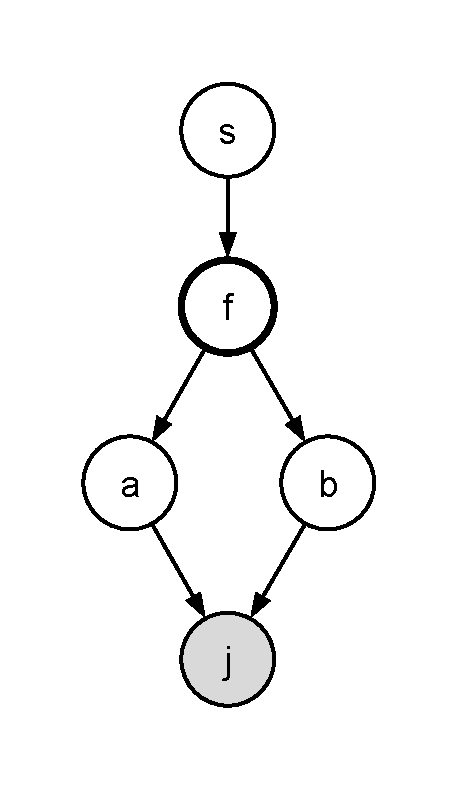
\includegraphics[height=36mm]{fig07_diamond_types/fig07a_induced.pdf}
    \caption{Two paths.}\label{fig:induced-a}
  \end{subfigure}\hfill
  \begin{subfigure}[b]{0.30\linewidth}\centering
    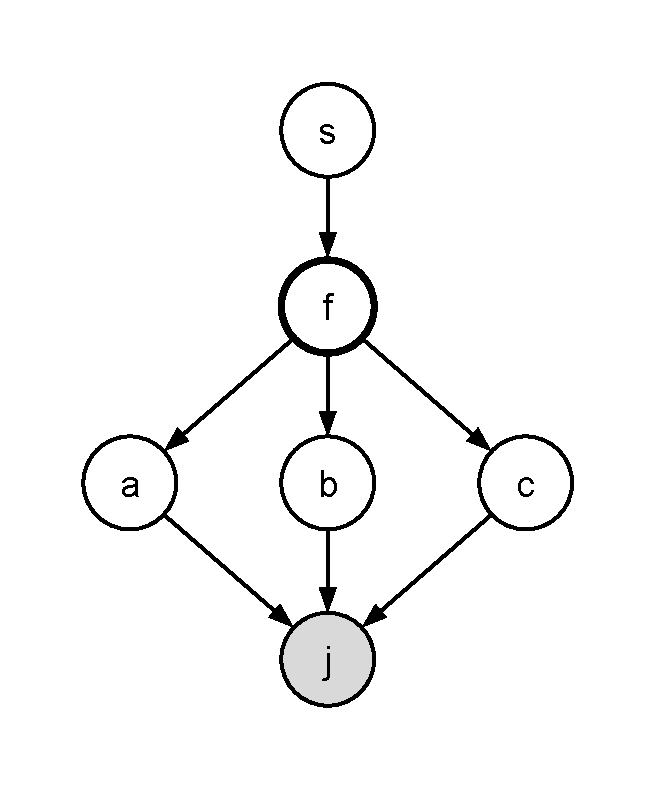
\includegraphics[height=36mm]{fig07_diamond_types/fig07e_induced3.pdf}
    \caption{Three paths.}\label{fig:induced-b}
  \end{subfigure}\hfill
  \begin{subfigure}[b]{0.34\linewidth}\centering
    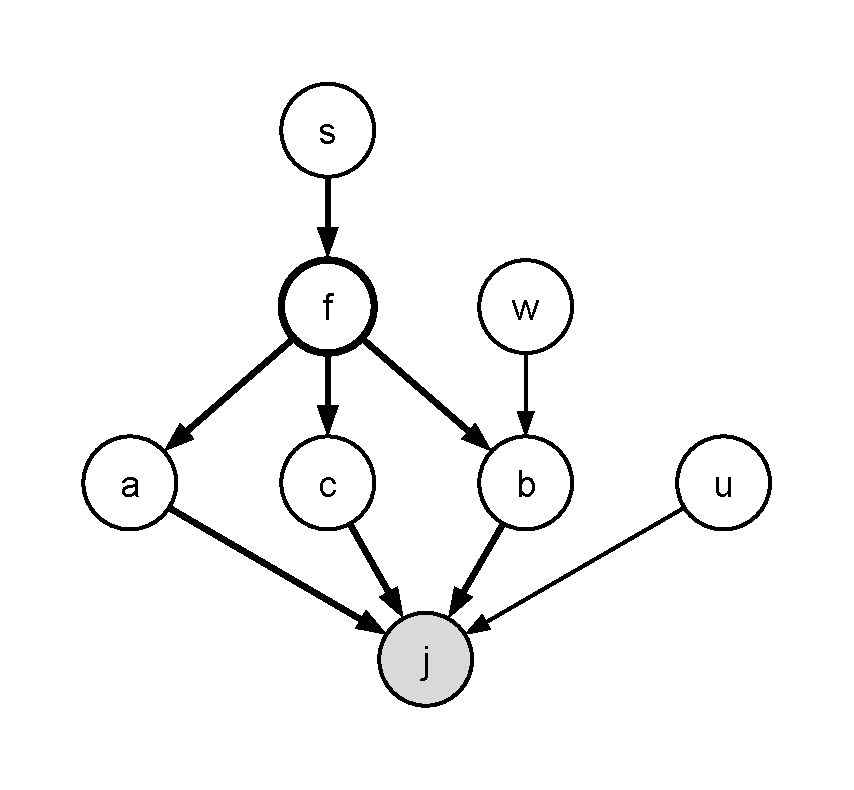
\includegraphics[height=42mm]{fig07_diamond_types/fig07f_induced_ext.pdf}
    \caption{With external edges.}\label{fig:induced-c}
  \end{subfigure}
  \caption{Induced diamonds. Every diamond path originates from the single fork and the subgraph carries one diamond join. }
  \label{fig:induced}
\end{figure}

\begin{figure}[htbp]
  \centering
  \begin{subfigure}[b]{0.30\linewidth}\centering
    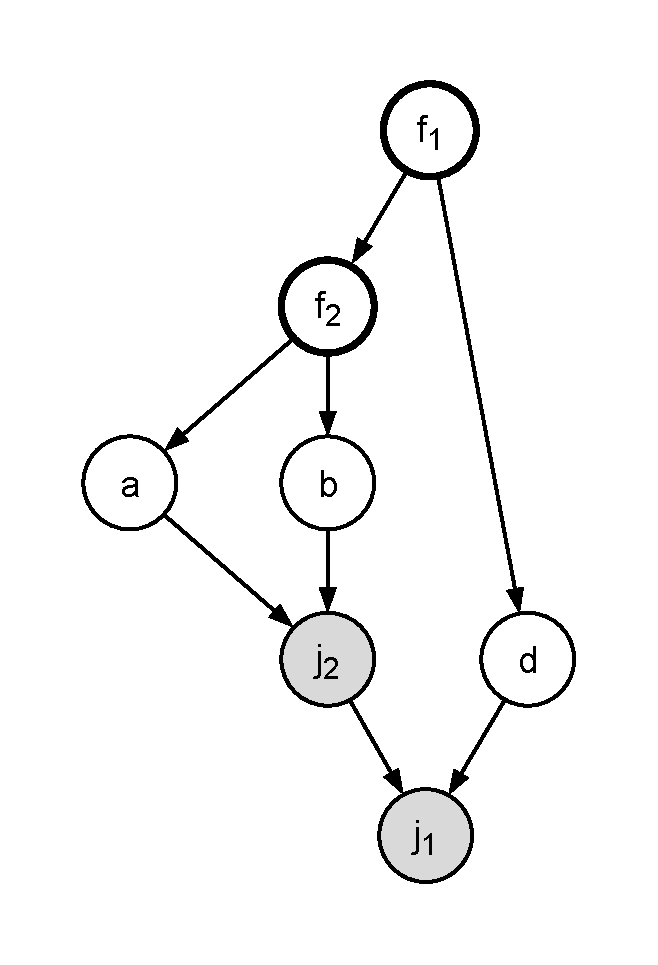
\includegraphics[height=42mm]{fig07_diamond_types/fig07c_nested.pdf}
    \caption{Nested.}\label{fig:noninduced-a}
  \end{subfigure}\hfill
  \begin{subfigure}[b]{0.30\linewidth}\centering
    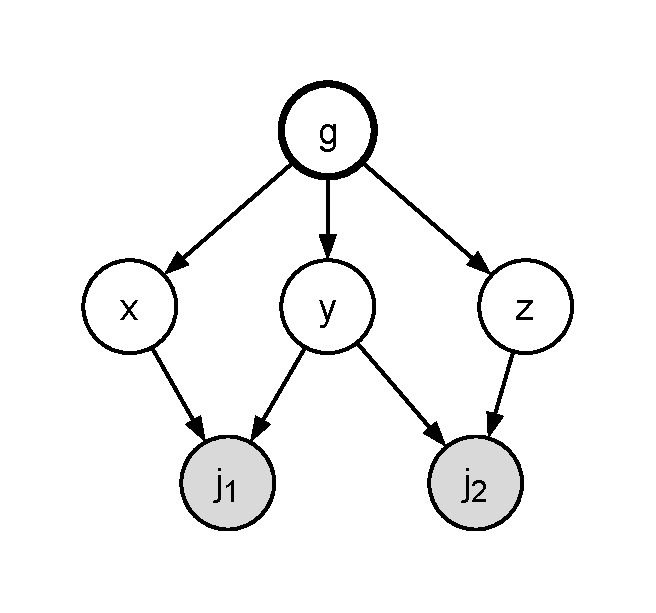
\includegraphics[height=36mm]{fig07_diamond_types/fig07d_shared.pdf}
    \caption{Overlapping.}\label{fig:noninduced-b}
  \end{subfigure}\hfill
  \begin{subfigure}[b]{0.34\linewidth}\centering
    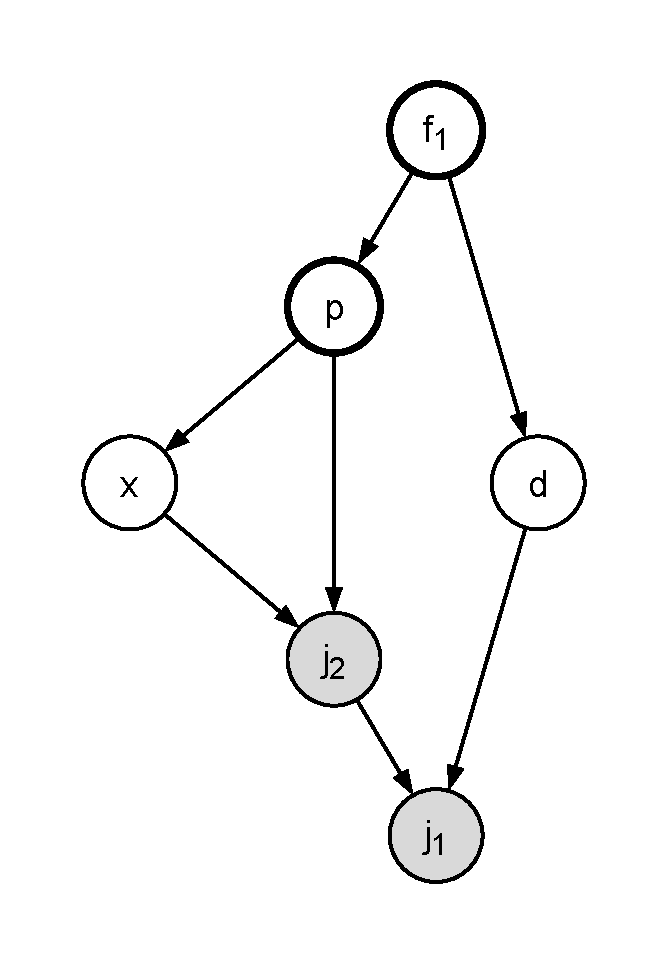
\includegraphics[height=42mm]{fig07_diamond_types/fig07g_selfinfl.pdf}
    \caption{Self-influencing, nested.}\label{fig:noninduced-c}
  \end{subfigure}
  \caption{Non-induced diamonds. In (b) two diamonds overlap through the shared fork $g$, and in (c) parent $p$ is itself the fork of the inner pattern.}
  \label{fig:noninduced}
\end{figure}

The decomposition module consumes the DAG $G=(V,E)$ and the iteration sets $L=\{L_1,\dots,L_k\}$ from the graph object of Chapter~\ref{ch:system-model}. Given the iteration sets, the topological index $\topi : V \to \{1,\dots,|V|\}$ follows by numbering nodes in increasing order across layers and in sorted node order within each layer, so every node receives a distinct integer and $\topi$ is a strict total order on $V$ refining the layered order.

The diamond in the framework is thus defined by the three discriminators.
\begin{itemize}
\item Eligibility criterion: the node's declared value must leave its reachability unsettled.
\item Anchoring structure: the shared fork from which the reconvergent paths originate.
\item Membership criterion: two parents belong to the same pattern when they share ancestry.
\end{itemize}

\label{sec:dd-isdet}
The eligibility criterion is the one discriminator not drawn from the diamond's definition, and \texttt{is\_det} in the implementation is the only place identification reads declared values. Since the module was built with probabilistic propagation in mind, the default eligibility criterion excludes nodes whose prior probability is deterministic. This covers two cases: any inactive node (i.e.\ unreachable with prior = $0$) or a perfect source node (i.e.\ always active with prior = $1$). The reason for the conjunction in the second case is that a non-source node with prior = $1$ may still be probabilistically uncertain, depending on its incoming edges. Therefore excluding every node valued $0$ or $1$ would incorrectly disable every diamond in a probabilistic DAG where all node priors happen to be $1$. For interval-valued and p-box-valued networks the two cases apply only to degenerate values, an interval or p-box collapsed exactly onto $0$ or $1$.

\begin{definition}[Diamond join]
\label{def:djoin}
A join node is a \emph{diamond join} when an unsettled fork lies in the shared ancestry of two of its parents, or one unsettled parent is itself an ancestor of another, so that a diamond forms there. A diamond join can itself be a fork of a different diamond elsewhere in the network.
\end{definition}

Each parent arriving at a diamond join carries its \emph{influencing set}, its ancestry under the self-inclusive closure, the nodes with a path to it and the parent itself. A diamond join can also receive paths that originate outside the fan-out, and these form its non-influencing set.

\begin{definition}[Non-influencing set]
\label{def:nondi}
The \emph{non-influencing set} of a diamond join is the set of its parents whose influencing sets meet no other parent's. Their edges enter the join from outside every reconvergent pattern there and are carried alongside the join's diamonds as independent contributions.
\end{definition}

Given this, the diamond subgraph is defined formally.

\begin{definition}[Diamond]
\label{def:diamond}
A diamond $D$ is a subgraph of $G$ whose relevant node set $R \subseteq V$ spans a diamond join, its correlated parents, and everything upstream of them, together with a set $C \subseteq V$ of fixed nodes that isolate the pattern.
\end{definition}

The framework exposes two views of the network's decomposed subgraphs.

\textbf{Unique diamonds} are the complete set of distinct diamonds found in the network, each stored once, in \texttt{unique\_subgraphs}. Any node can participate in any number of unique diamonds, whether as a fan-out point, a fan-in point, or an intermediate node along the paths.

\textbf{The maximal diamond} is the network-level view of a diamond join. It is the full subgraph the join's reconvergence forms, made up of the diamond of every group of the join's parents that forms one, spanning the join, the groups, and everything upstream of them, together with the edges of the join's non-influencing set. Therefore every diamond join has at most one maximal diamond, while a fork can participate in several. Every diamond found at a deeper level inside a maximal diamond is a \textbf{sub-diamond}, and its edge list is contained in the enclosing diamond's.

Two consequences follow from these definitions. A unique diamond with no inner sub-diamond has one fork and one diamond join, so it is an induced diamond, the smallest a diamond can be. Furthermore, since every diamond is either maximal at its join or a sub-diamond of a maximal one, the set of unique diamonds is the set of distinct maximal diamonds together with their inner sub-diamonds.

\section{The Identification Algorithm}
\label{sec:dd-algorithm}

\texttt{identify\_diamonds} is a recursive set-membership algorithm over the closures of the graph object. For every join node of $G$ it identifies the join's maximal diamond, pairing the join with the earliest covering forks in its parents' shared ancestry, and it recurses inside each diamond it forms for the sub-diamonds. Each call works on a join $v$, a \emph{fixed context} $E \subseteq V$ of nodes already fixed by enclosing diamonds, and the parents $P$ of $v$ in view. The recursion starts from $E = \varnothing$, and Algorithm~\ref{alg:new-identify} shows the skeleton.

Under a context each parent's influencing set shrinks to
\[
\infl(p,E) \;=\; \Anc(p)\setminus E ,
\]
with $\Anc(p)$ self-inclusive so that $p \in \infl(p,E)$ whenever $p \notin E$. Two parents $p, q$ of a join are \emph{structurally correlated under $E$} when $\infl(p,E) \cap \infl(q,E) \neq \varnothing$, that is, when some node upstream of both is not held fixed. Similar to factoring based decomposition, extending the context with a node removes it from every influencing set.

\begin{algorithm}[htbp]
\caption{Recursive diamond identification (skeleton)}
\label{alg:new-identify}
\begin{algorithmic}[1]
\Require join node $v$, fixed context $E$, parents $P$ of $v$ in view
\Ensure the diamonds at $v$ under $E$
\State partition $P$ into groups by pairwise influencing-set intersection
\ForAll{groups $G$ with $|G| \geq 2$}
    \State $f \gets$ eligible covering fork of $G$ with minimum $\topi$
    \If{no eligible covering fork exists}
        \State members of $G$ join the non-influencing set of $v$; skip the group
    \EndIf
    \State build diamond $D$ for $(v, G, f)$ under $B = E \cup \{f\}$
    \State reuse the stored entry if the identity key of $D$ is already in \texttt{unique\_subgraphs}
    \ForAll{join nodes $j$ within $D$}
        \State recurse on $(j, B, \text{parents of } j)$, restricted to $G$ when $j = v$
    \EndFor
\EndFor
\State singleton groups join the non-influencing set of $v$
\end{algorithmic}
\end{algorithm}

\subsection{Shared ancestry and the earliest covering fork}
\label{sec:dd-partition}
\label{sec:dd-fork}

At a join $v$ with parents $P$ under context $E$, any two parents whose influencing sets intersect are merged into one group by union--find.

\begin{theorem}[Grouping correctness]
\label{thm:grouping}
Fix a join $v$, context $E$, and parent set $P$. Let $H$ be the undirected graph on vertex set $P$ with an edge between $p$ and $q$ if and only if $\infl(p,E) \cap \infl(q,E) \neq \varnothing$. Then \texttt{components}$(P,E)$ returns exactly the connected components of $H$.
\end{theorem}

\begin{proof}
The intersection $\infl(p,E) \cap \infl(q,E)$ is evaluated for every unordered pair of $P$, so the pairs that intersect are exactly the edges of $H$, and union--find merges exactly those pairs. Union--find over a vertex set and its edge relation returns the connected components, which for $P$ under this edge relation is the component partition of $H$.
\end{proof}

\begin{theorem}[Group disjointness]
\label{thm:disjoint}
If $G_i \neq G_j$ are distinct groups returned by \texttt{components}$(P,E)$, then
\[
\Bigl(\bigcup_{p\in G_i}\infl(p,E)\Bigr) \;\cap\; \Bigl(\bigcup_{q\in G_j}\infl(q,E)\Bigr) \;=\; \varnothing .
\]
\end{theorem}

\begin{proof}
Let $p \in G_i$ and $q \in G_j$. By Theorem~\ref{thm:grouping} they lie in different components of $H$, and since every pair was evaluated, $\infl(p,E) \cap \infl(q,E) = \varnothing$. The intersection of the two unions expands to the union of these pairwise intersections, each of which is empty.
\end{proof}

Disjointness here is a statement about the influencing sets of the diamond groups, namely that each group decomposes separately. Whether separately computed values recombine correctly at the join is a different claim, which Chapter~\ref{ch:probability-toolkit} makes and proves for the probabilistic reading. Parents in singleton groups fall into the join's non-influencing set.

Each group of two or more is then searched for its eligible covering forks, those lying in the shared ancestry of at least two members and not already in the fixed context, with a member that is an ancestor of another counting as its own cover. The diamond anchors on the earliest of them, the covering fork of minimum topological index, which leaves the largest part of the group's shared structure intact downstream for reuse, and the strict total order makes the choice unique. A group whose shared ancestry offers no eligible covering fork forms no diamond, and its members join the non-influencing set.

\subsection{Recursive flow}
\label{sec:dd-loop}

\begin{theorem}[Termination]
\label{thm:termination}
The recursion of Algorithm~\ref{alg:new-identify} terminates after at most $|V|$ nested context extensions along any recursive path.
\end{theorem}

\begin{proof}
Along any path of the recursion, each call either returns without recursing, which happens when every group at the join in view is a singleton or offers no covering fork, or fixes a fork $f$ and recurses with $B = E \cup \{f\}$. Covering forks are never already in $E$ (Section~\ref{sec:dd-fork}), so $f \notin E$ and $|V \setminus B| = |V \setminus E| - 1$ strictly. The quantity $|V \setminus E|$ is a non-negative integer that strictly decreases along the recursive path, and from its initial value $|V \setminus \varnothing| = |V|$ it admits at most $|V|$ decrements.
\end{proof}

Fixing fork $f$ for group $G$ at join $v$ yields the diamond with boundary $B = E \cup \{f\}$. Paths within the diamond can share further unfixed ancestry, so the recursion runs again at every join within it, the diamond join itself included, under the extended context. Sub-diamonds form inside maximal diamonds this way until no covering fork and join pair remains anywhere.

\subsection{Subgraph construction}
\label{sec:dd-edges}

The diamond for group $G$ at join $v$ under boundary $B$ spans
\[
R \;=\; \{v\} \cup G \cup \bigcup_{p \in G}\Anc(p),
\]
the join, the group, and everything upstream of the group, with induced edge list
\[
\ED \;=\; \bigl\{\, (u,w) \in E \;:\; u,w \in R,\;\; w \notin B,\;\; (w \neq v \;\text{or}\; u \in G) \,\bigr\}.
\]
Write $V(\ED)$ for the set of its endpoints. The first two clauses keep the edge list on the relevant set $R$. The third removes every edge into a fixed node, whose upstream structure is already settled, while its outgoing edges stay and act as local sources of the diamond. The fourth admits an edge into the diamond join only from the group. The reason for the fourth clause is given after the lemma.

\begin{lemma}[Edge isolation]
\label{lem:isolation}
Let $D$ be constructed for group $G$ at join $v$ under boundary $B$ as above. Then $(u,w) \in \ED$ if and only if $(u,w)\in E$, $u,w \in R$, $w \notin B$, and ($w \neq v$ or $u \in G$). Consequently every directed path within $\ED$ that terminates at $v$ has its final edge originating in $G$, and no node of $B$ appears on any path within $\ED$ except as its first node.
\end{lemma}

\begin{proof}
The membership characterisation restates the filter defining $\ED$. For the path properties, induct on path length. A length-one path into $v$ is a single edge $(u,v) \in \ED$, which the fourth clause forces to have $u \in G$. Any longer path has a final edge satisfying the same property, and each preceding edge $(u,w)$ has $w \notin B$ and both endpoints in $R$ by the first three clauses, so no node after the first lies in $B$ and no edge of the path enters from outside $R$.
\end{proof}

Consider a nested level at which an enclosing diamond has already fixed a fork $r$, so $r \in E$, and suppose $r$ is both an ancestor of some group member $p$ and a direct parent of the join $v$. Partitioning places $r$ correctly, since fixing removed $r$ from every influencing set, and in the minimal case of $r$ a source with no free ancestry its influencing set is empty, landing it in a singleton group whose contribution to $v$ enters separately.

However, the span $R$ is built from the raw closure $\Anc(p)$ and contains $r$ whatever the context says, so the partition and the span disagree wherever $E \neq \varnothing$. The edge $(r,v)$ then has both endpoints in $R$ and a head outside $B$, so the first three clauses admit it, and a diamond meant to capture $v$ as reached through $G$ alone gains a second, unrelated entry into its own join. The fourth clause blocks this edge. Figure~\ref{fig:isolation} shows the minimal instance.

\begin{figure}[htbp]
  \centering
  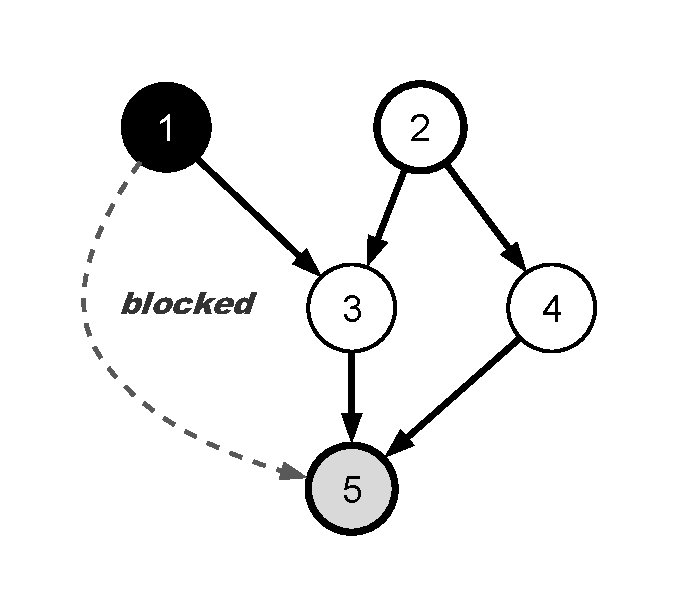
\includegraphics[width=0.42\linewidth]{fig06_edge_isolation/fig06_edge_isolation.pdf}
  \caption[Edge isolation at a nested join]{Edge isolation at join 5 in context $E=\{1\}$. Node 1 (filled) was fixed by an enclosing diamond and is excluded from the group $G=\{3,4\}$ with fork 2. Its direct edge $(1,5)$, drawn dashed, is admitted by the first three filter clauses but blocked by the fourth. Bold edges form the nested diamond's edge list.}
  \label{fig:isolation}
\end{figure}

\subsection{Context-aware identity}
\label{sec:dd-identity}

A diamond's edge list alone cannot place it in the nesting hierarchy.

\begin{proposition}
\label{prop:identity}
(i) There exist graphs and contexts $E_A = \varnothing$ and $E_B = \{g\}$, with $g$ a source fork among the endpoints of $\ED$, under which the construction of Section~\ref{sec:dd-edges} anchors the same fork $f$ and yields the same edge list $\ED$, while one diamond is maximal and the other a sub-diamond. The pair $(\ED, \{f\})$ therefore conflates distinct diamonds. (ii) Under $\hkey(D) = (\ED, \{f\}\cup(E\cap V(\ED)))$, equal keys imply the same diamond join, the same group, the same edge list, and the same set $C$, with the two fixed contexts agreeing on every node of $V(\ED)$ and every stored field equal.
\end{proposition}

\begin{proof}
For (i), take a join $v$ whose group $G$ anchors on fork $f$, and a source fork $g$ that is an ancestor of exactly one member of $G$ and keeps one edge whose head lies outside both boundaries. Coverage of one excludes $g$ from the covering-fork search, so the search offers the same forks in both cases and $f$ is anchored in both, and removing $g$ from a single influencing set cannot split the group, since the correlation runs through $f$. The cut into $g$ removes nothing, as a source has no incoming edges, and $g$'s retained edge passes the filter in both cases, so $g \in V(\ED)$. The group, the fork, the span, and the edge list therefore coincide, while the diamond is maximal under $E_A$ and a sub-diamond of the one that fixed $g$ under $E_B$. The keys differ, since $E_A \cap V(\ED) = \varnothing$ and $g \in E_B \cap V(\ED)$.

For (ii), equal keys give equal $\ED$ and equal $C$, since both are hashed. The diamond join is recoverable as the unique endpoint of $\ED$ that every other endpoint precedes in the closure, which acyclicity makes unique, and the group as the in-neighbourhood of the join in $\ED$, which the fourth clause admits from the group alone. Every stored field is computed from $\ED$, $V(\ED)$, $C$, and the global closures, so equal inputs give equal fields, and $B\cap V(\ED) = (\{f\}\cap V(\ED)) \cup (E\cap V(\ED)) = C \cap V(\ED)$ in both constructions. The two fixed contexts can still disagree away from the diamond, but only narrowly. A node outside the span is never consulted, since every membership test in the recursion concerns a parent of a join within the diamond or one of its ancestors, all inside the span by transitivity. A span node $x$ in one fixed context and not the other has no incoming edge, since such an edge would have its tail in the span and would pass the filter where $x$ is free, forcing $x \in V(\ED)$, and each outgoing edge of $x$ inside the span is absent from the shared $\ED$, so its head lies in each construction's boundary or it is a direct edge into the join excluded by the fourth clause. Every path from such a node towards the diamond therefore begins at a node in both fixed contexts or at an excluded edge.
\end{proof}

Since a diamond cannot be unique by its edge list and fork alone, every unique diamond is keyed by
\[
\hkey(D) \;=\; \bigl(\ED,\; \{f\} \cup (E \cap V(\ED))\bigr) ,
\]
where $\ED$ is the diamond's edge list, $f$ its covering fork, and $E \cap V(\ED)$ the fixed context restricted to the diamond's endpoints.

\label{sec:dd-hashconsing}
Before a new entry is built, the key is looked up in \texttt{unique\_subgraphs}, and a structurally identical diamond already resolved anywhere in the recursion is referenced instead of rebuilt. This is hash-consing \cite{ershov1958programming,filliatre2006hashconsing}, a table keyed by structural identity so that equal structures are stored once and identity comparison becomes a key comparison, sometimes used in BDD algorithms. Without the store the recursion is a tree and every call site is distinct. With it, structurally identical call sites collapse into shared entries and the representation becomes a DAG. Diamonds with the same identity share one stored entry regardless of the outer context, since Proposition~\ref{prop:identity} bounds whatever influence a node outside the identity carries towards the diamond, and the shared entry meets the same fixed context within.

\section{Structural Correctness}
\label{sec:dd-correctness}

\subsection{Global completeness}

\begin{theorem}[Global completeness]
\label{thm:completeness}
Let $v$ be a join node of $G$ with parent set $P$, and suppose there exist distinct $p, q \in P$ and an unsettled node $a$ such that either $a$ is a fork node in $\Anc(p)\cap\Anc(q)$, or $p \in \Anc(q)$ (the asymmetric case, taking $a = p$). Then the top-level pass of \texttt{identify\_diamonds} stores a maximal diamond for $v$. Conversely, a join admitting no such pair receives none.
\end{theorem}

\begin{proof}
At the top level $E = \varnothing$, so in either case $a \in \infl(p,\varnothing)\cap\infl(q,\varnothing)$ and the intersection is non-empty. By Theorem~\ref{thm:grouping}, $p$ and $q$ lie in a common group $G$ with $|G|\ge 2$. In the covering-fork search, $a$ counts once for each member it covers. In the symmetric case $a$ is a fork in both ancestries and covers $p$ and $q$. In the asymmetric case $a = p$ is necessarily a fork, since it has an edge to $v$ and a path to $q$ that cannot pass through $v$, and with the self-inclusive closure it covers itself as well as $q$. Either way the coverage reaches $2$ and the set of covering forks is non-empty. A non-empty finite set has a $\topi$-minimal element, so the search anchors some fork, not necessarily $a$ itself, Algorithm~\ref{alg:new-identify} constructs a diamond for $G$, and the top-level pass records it under $v$. For the converse, suppose no such pair exists. Any covering fork the search admits would yield one, since a symmetric cover is a fork in two members' ancestries, an asymmetric cover is a parent in another member's ancestry, and the search admits only unsettled nodes. Every group therefore offers no covering fork, whether its members are unrelated or related only through settled structure, and the algorithm constructs nothing at $v$. That is the correct outcome, because whatever shared ancestry remains at $v$ is already settled.
\end{proof}

\subsection{Determinism}

\begin{theorem}[Determinism]
\label{thm:determinism}
For a fixed input graph and iteration sets $(G, L)$, join $v$, context $E$, and admissible parent set, the diamonds returned by Algorithm~\ref{alg:new-identify} are uniquely determined, independent of set or dictionary iteration order, thread scheduling, or any other accident of execution.
\end{theorem}

\begin{proof}
By induction on recursion depth, it suffices that each step of one call is a function of its arguments alone. This holds for the partition step because, by Theorem~\ref{thm:grouping}, its output is the connected-component partition of $H$, a graph invariant that does not depend on the order in which pairs are examined or merges performed. It holds for the selection step because the set of covering forks is itself a function of the arguments, and either it is empty, in which case the group deterministically produces no diamond, or the diamond anchors on its minimum under $\topi$, which a strict total order makes unique. The boundary $B = E \cup \{f\}$ and span $R$ are then determined, hence so is $\ED$, and hence so are the joins passed to the recursive calls, which are deterministic by the inductive hypothesis. The store adds one further mechanism, reuse of an earlier entry on a key hit. Proposition~\ref{prop:identity}(ii) makes equal keys carry the same join, group, edge list, and stored fields, and confines any residual difference between merged call sites to nodes outside the identity, so reuse introduces no dependence on visit order.
\end{proof}

This guarantee is similar to the canonicity guarantee of reduced ordered binary decision diagrams \cite{bryant1986graph}. While BDD canonicity depends on an externally supplied variable ordering, $\topi$ is derived from a property of the input graph.

\section{The Unique Diamond Object}
\label{sec:dd-representation}
\label{sec:dd-selfsimilar}

The algorithm builds each unique diamond as a graph object of its own. The unique diamond object carries the diamond's characteristics together with its subgraph in the same form as the network's graph object, so a diamond can be treated as a standalone DAG network for any other type of analysis in the framework. Table~\ref{tab:dd-selfsimilar} lists its fields.

\begin{table}[htbp]
\centering
\caption{Fields of the unique diamond object}
\label{tab:dd-selfsimilar}
\small
\renewcommand{\arraystretch}{1.15}
\begin{tabular}{|l|p{0.55\textwidth}|}
\hline
\textbf{Field} & \textbf{Role} \\
\hline
\texttt{sub\_outgoing\_index} & Forward adjacency of the diamond \\
\texttt{sub\_incoming\_index} & Reverse adjacency of the diamond \\
\texttt{sub\_sources} & Local sources \\
\texttt{sub\_fork\_nodes} & Local forks \\
\texttt{sub\_join\_nodes} & Local joins \\
\texttt{sub\_ancestors} & Ancestor closure restricted to the diamond's nodes \\
\texttt{sub\_descendants} & Descendant closure restricted to the diamond's nodes \\
\texttt{sub\_iteration\_sets} & Layered order restricted to the diamond's nodes \\
\texttt{sub\_node\_priors} & Value map restricted to the diamond's nodes \\
\texttt{sub\_diamond\_structures} & For each join within this diamond, its sub-diamonds, held by their keys into \texttt{unique\_subgraphs}, and its non-influencing set \\
\texttt{is\_maximal} & Whether the diamond is maximal \\
\texttt{diamond} & The span $R$, the set $C$, and the edge list $\ED$ \\
\hline
\end{tabular}
\end{table}

Invoking the decomposition module on the graph object of Chapter~\ref{ch:system-model} extends the object with the field \texttt{unique\_subgraphs}, holding the network's unique subgraphs. The Probability Propagation Algorithm of Chapter~\ref{ch:probability-toolkit} reduces each solved diamond to a supernode. The concrete Julia types behind the fields of Table~\ref{tab:dd-selfsimilar} are described in Chapter~\ref{ch:julia-package}.

\section{Worked Examples}
\label{sec:dd-examples}

\subsection{The induced diamond}
\label{sec:dd-atomic}

Figure~\ref{fig:induced-a} is the minimal pattern, a source $s$ feeding a fork $f$, two internally disjoint paths, and a join $j$ where they meet. At $j$ both parents' influencing sets contain $f$, so the parents form one group. Fork $f$ is the only covering fork and is fixed, and the diamond spans the whole figure with $C = \{f\}$.


\subsection{A factorised join}
\label{sec:dd-factorised-example}

The nine-edge network of Figure~\ref{fig:factorised} has forks 1 and 2 and a single join at node 7, which source 8 also feeds directly. The parents split into two correlated groups, $\{3,4\}$ through fork 1 and $\{5,6\}$ through fork 2, with parent 8 related to neither. Two constituent diamonds arrive at join 7, one anchored on each fork, and node 8 is carried in the non-influencing set. Together they are the join's maximal diamond.

\begin{figure}[htbp]
  \centering
  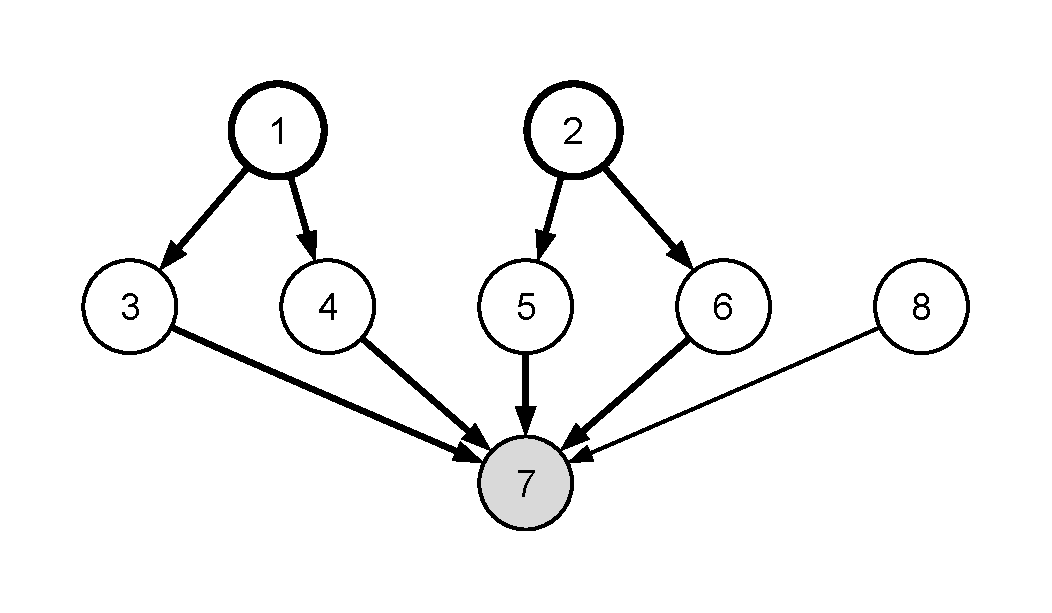
\includegraphics[width=0.42\linewidth]{fig08_factorised/fig08_factorised.pdf}
  \caption{A factorised join. Two correlated groups meet at join 7, one through each fork, and source 8 enters from outside both. Bold edges mark the two constituent diamonds.}
  \label{fig:factorised}
\end{figure}
\subsection{A nested decomposition}
\label{sec:dd-nested-example}

The eight-node network of Figure~\ref{fig:nested-full} has forks 1 and 3 and joins 6 and 8. An outer reconvergence runs through fork 1 and meets at join 8, and on one of its branches an inner reconvergence runs through fork 3 and meets at join 6. The decomposition below is the machine-checked output of the implementation on this edge list, and the examples of Figures~\ref{fig:isolation} and~\ref{fig:factorised} were verified in the same run.

\begin{figure}[htbp]
  \centering
  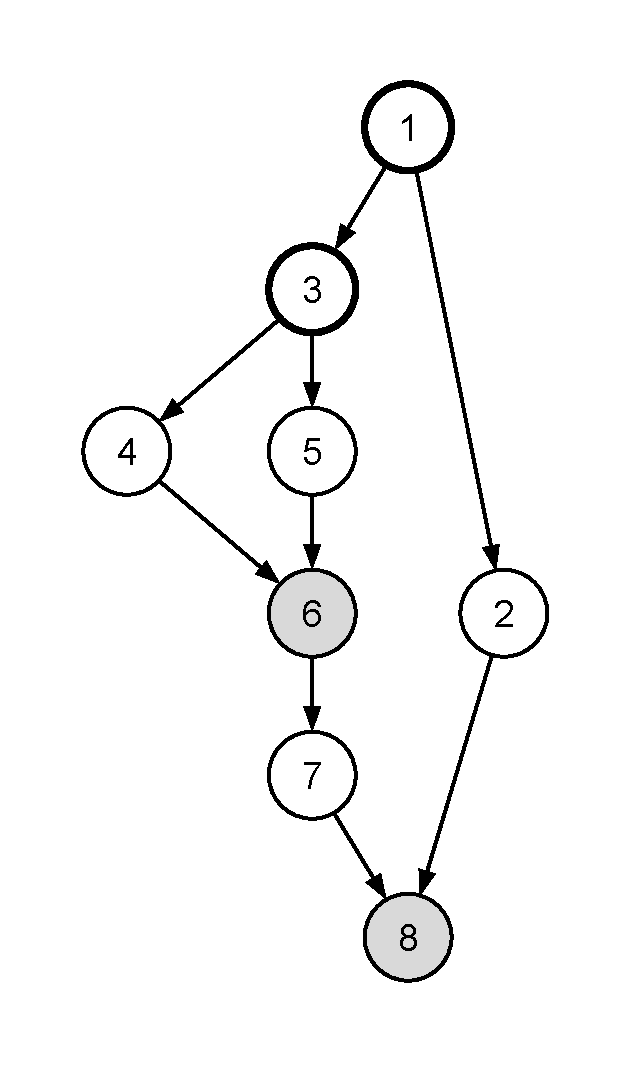
\includegraphics[width=0.34\linewidth]{fig02_nested_full/fig02_nested_full.pdf}
  \caption{Frame 1. The network, with forks outlined in bold and joins shaded.}
  \label{fig:nested-full}
\end{figure}

\textbf{Join 8, top level.} The parents are $\{2,7\}$, with $\infl(2,\varnothing) = \{1,2\}$ and $\infl(7,\varnothing) = \{1,3,4,5,6,7\}$. The sets intersect in $\{1\}$, so the parents form one group. Fork 1 is the only covering fork of the pair and is fixed, and the maximal diamond $D_1$ spans all nine edges with $C = \{1\}$ (Figure~\ref{fig:nested-outer}).

\begin{figure}[htbp]
  \centering
  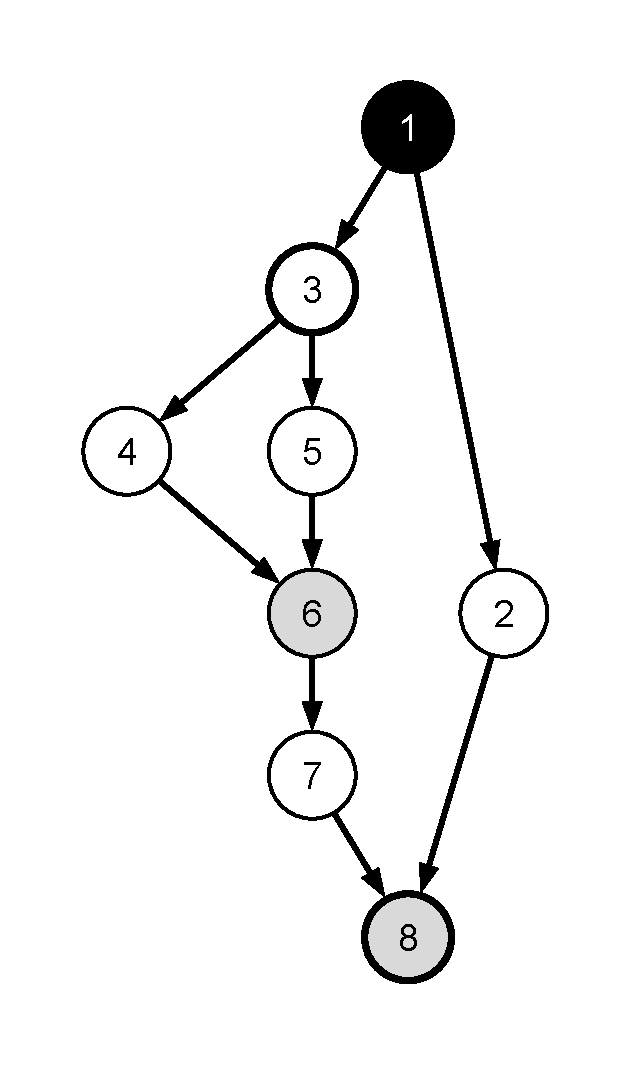
\includegraphics[width=0.36\linewidth]{fig03_nested_outer/fig03_nested_outer.pdf}
  \caption{Frame 2. The maximal diamond at join 8, with fork 1 fixed (filled) and the span covering the whole network.}
  \label{fig:nested-outer}
\end{figure}

\textbf{Join 6, inside $D_1$.} Under the boundary $B = \{1\}$, join 6 has parents $\{4,5\}$ with $\infl(4,\{1\}) = \{3,4\}$ and $\infl(5,\{1\}) = \{3,5\}$. The parents are still correlated through fork 3, so fixing 1 did not resolve the inner reconvergence. The recursive call fixes fork 3 and produces the inner diamond $D_3$ with $C = \{3\}$ and $\ED = \{(3,4),(3,5),(4,6),(5,6)\}$. The edge $(1,3)$ is cut by the boundary clause because its head is fixed at this level (Figure~\ref{fig:nested-inner}).

\begin{figure}[htbp]
  \centering
  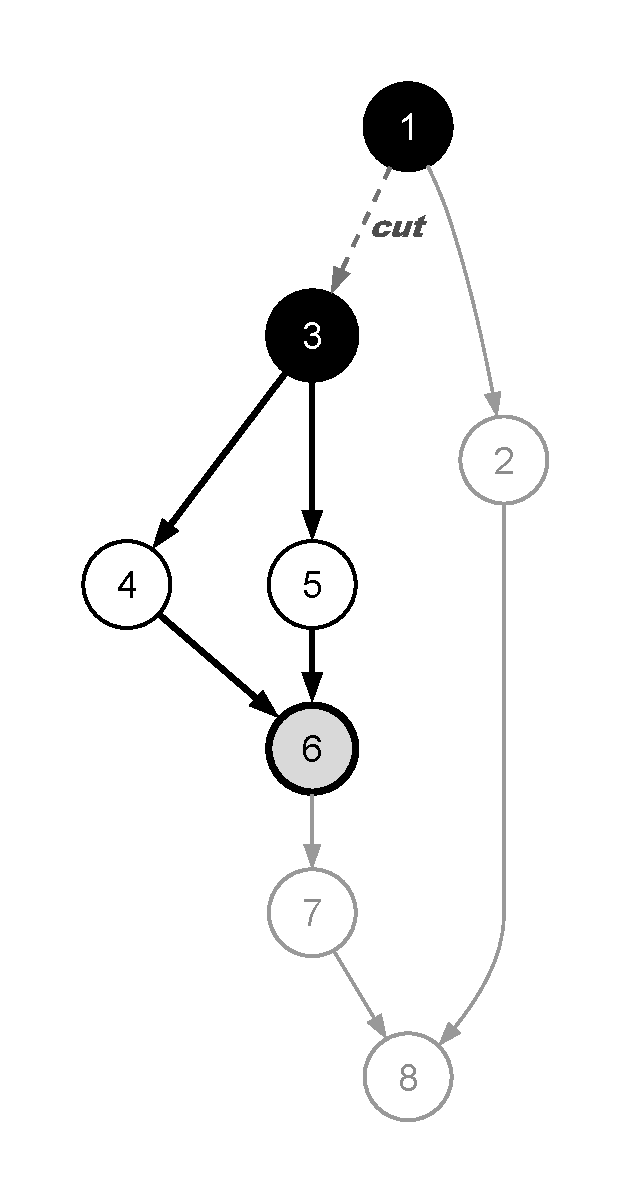
\includegraphics[width=0.36\linewidth]{fig04_nested_inner/fig04_nested_inner.pdf}
  \caption{Frame 3. The recursive call at join 6 in context $E=\{1\}$, with fork 3 fixed, the inner diamond in bold, and edge $(1,3)$ cut.}
  \label{fig:nested-inner}
\end{figure}

\textbf{Join 6, top level.} Join 6 is also a join of the network itself, so the top-level pass visits it in its own right. With $E = \varnothing$, forks 1 and 3 both cover parents 4 and 5, and the earliest covering fork rule fixes fork 1 and not fork 3. The result is a second maximal diamond $D_2$ spanning $\{(1,3),(3,4),(3,5),(4,6),(5,6)\}$ with $C = \{1\}$, and the recursion inside it, now in context $\{1\}$, again produces exactly $D_3$.

\textbf{The emitted hierarchy.} In total the module returns two maximal diamonds and three unique diamonds (Figure~\ref{fig:hierarchy}). $D_1$ sits at join 8 and $D_2$ at join 6, each with $C=\{1\}$. The inner $D_3$ at join 6 with $C=\{3\}$ is stored once and referenced from the substructure tables of both $D_1$ and $D_2$ under the same key. Two different enclosing recursions posed the same sub-problem, with the same edge list, the same fork, and contexts agreeing on the span. Proposition~\ref{prop:identity}(ii) is the reason the single shared entry is correct.

\begin{figure}[htbp]
  \centering
  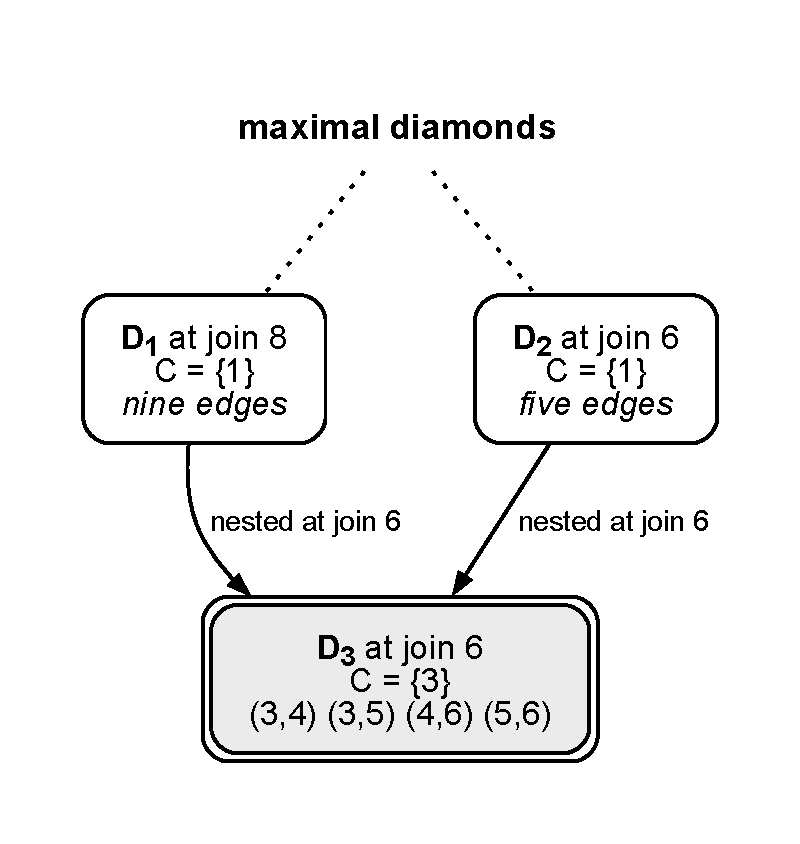
\includegraphics[width=0.6\linewidth]{fig05_hierarchy/fig05_hierarchy.pdf}
  \caption{Frame 4. The emitted hierarchy of two maximal diamonds, with the inner diamond $D_3$ stored once and referenced by both.}
  \label{fig:hierarchy}
\end{figure}

The trace also confirms the edge-isolation case of Section~\ref{sec:dd-edges} end to end. In the network of Figure~\ref{fig:isolation}, the nested diamond at join 5 under $E=\{1\}$ is emitted with $C = \{2\}\cup(\{1\}\cap V(\ED)) = \{1,2\}$, node 1 staying among the edge list's endpoints through its surviving edge $(1,3)$, which is the context-aware identity of Section~\ref{sec:dd-identity} visible in the output. Node 1 is recorded in the nested diamond's non-influencing set, and the edge $(1,5)$ appears nowhere in its edge list. At the top level node 1 is a member of the group itself, so the maximal diamond at join 5 carries $(1,5)$ legitimately.


\section{Summary}
\label{sec:dd-summary}

The module extends the graph object of Chapter~\ref{ch:system-model} with \texttt{unique\_subgraphs}, storing every diamond found at any level exactly once, each entry a graph object of the same form as the network it came from, with the maximal diamonds flagged. The decomposition terminates within $|V|$ nested steps and is canonical for a given input (Theorems~\ref{thm:termination} and~\ref{thm:determinism}). It groups a join's parents exactly by shared unfixed ancestry and produces a diamond wherever unsettled reconvergence exists and only there (Theorems~\ref{thm:grouping}--\ref{thm:completeness}). Nothing outside a diamond's span enters its edge list (Lemma~\ref{lem:isolation}), and the context-aware identity of Section~\ref{sec:dd-identity} distinguishes a maximal diamond from a sub-diamond with the same edge list and fork (Proposition~\ref{prop:identity}).

\ifdefined\maindoc
% do nothing
\else
\printbibliography
\end{document}
\fi